\documentclass[conference]{IEEEtran}
\IEEEoverridecommandlockouts
% The preceding line is only needed to identify funding in the first footnote. If that is unneeded, please comment it out.
\usepackage{cite}
\usepackage{amsmath,amssymb,amsfonts}
\usepackage{algorithmic}
\usepackage{graphicx}
\usepackage{textcomp}
\def\BibTeX{{\rm B\kern-.05em{\sc i\kern-.025em b}\kern-.08em
    T\kern-.1667em\lower.7ex\hbox{E}\kern-.125emX}}
\begin{document}

\title{Adversarially-Robust Minimal DeFi Agent For Cryptocurrency Swapping}

\author{\IEEEauthorblockN{Biying FANG (ID:12341000)\IEEEauthorrefmark{1}, Yifan LI (ID:12341000)\IEEEauthorrefmark{1}, Mengmeng SU (ID:59669920)\IEEEauthorrefmark{1}, \\ Siqi SUN (ID:59414589)\IEEEauthorrefmark{1} and Tsz Chun TSOI (ID:57159984)\IEEEauthorrefmark{1}} 
\IEEEauthorblockA{\IEEEauthorrefmark{1}College of Computer Science\\
City University of Hong Kong, Tat Chee Avenue, Kowloon, Hong Kong SAR\\
Email: tszctsoi4-c@my.cityu.edu.hk} }


\maketitle


\section{Introduction}
The user interfaces of Decentralized Finance (DeFi) are shifting from manually manipulating discrete transactions on‐chains to delegating these tasks to conversational agents and AI‑augmented intermediaries, ranging from wallet‑embedded copilots, Telegram‑based trading bots, to fully autonomous DeFi assistants. These systems convert natural‑language directives into executable blockchain operations, effectively inserting a probabilistic planning layer into what was a deterministic pipeline under user's control.

The shift introduces a qualitatively distinct and insufficiently studied security boundary. In contrast to explicit and formally analyzable smart contracts, large language models (LLMs) exhibit stochasticity and are susceptible to various linguistic and contextual adversarial actions, including prompt injection, indirect influence attacks, contextual contamination, and social‑engineering‑driven specification drift. The threat is particularly apparent in open multi‑party communication environments such as Telegram or WhatsApp, where adversaries may directly interact with the same agent instance as the legitimate user, embedding payloads designed to subvert the transaction‑generation process.

Considering the irreversibility of blockchain transactions, compromised transaction plan or signing key can result in catastrophic and permanent asset loss. Still, while existing literature extensively investigates vulnerabilities in smart‑contract correctness, MEV extraction dynamics, oracle manipulation, and private‑key security, there exists a notable absence of empirical and systematic analysis addressing the security properties of LLM‑driven transaction‑planning pipelines under adversarial language conditions. The research aims to fill the said gaps at the intersection of natural‑language AI systems and decentralized financial infrastructure by implementing and testing a minimal prototype.



\section{Application Setting}

\subsection{System Architecture}
Guidelines: In this subsection, you should describe the general application setting of encrypted search, e.g., how many parties are there in the real application setting, the particular role of each party, and the participation of each party (i.e., what each party does in  the work flow).

\subsection{Threat Model}

Guidelines: In this subsection, you should explain the threat assumptions generally adopted by the literature on encrypted search. For example, you may clearly indicate the trust assumptions of each party involved in the application (i.e., who is trusted or untrusted?), the goal of the untrusted party (e.g., what does the adversary want to learn?), how the adversary will behave, in a semi-honest fashion or in a malicious manner?


\begin{table}[h]
\centering
\caption{Comparison of encrypted search schemes.}
\label{my-label}
\begin{tabular}{|l|l|l|}
\hline
Scheme & Search Complexity & Index Size \\ \hline
\cite{SongWP00}   & ...              & ...       \\ \hline
...    & ...               & ...        \\ \hline
\end{tabular}
\end{table}


\section{Research Directions of Encrypted Search}
%

Guidelines: In this subsection, you should introduce the typical research directions for encrypted search, describe in detail the goals of each research direction in terms of functionality and/or security. You should also specify and discuss the design challenges in each direction based on your literature study and or your personal perspectives. Besides, you should properly discuss the existing works and try to reflect the state-of-the-art. A possible organization structure is given below. 


\begin{figure}[!t]
  \centering
  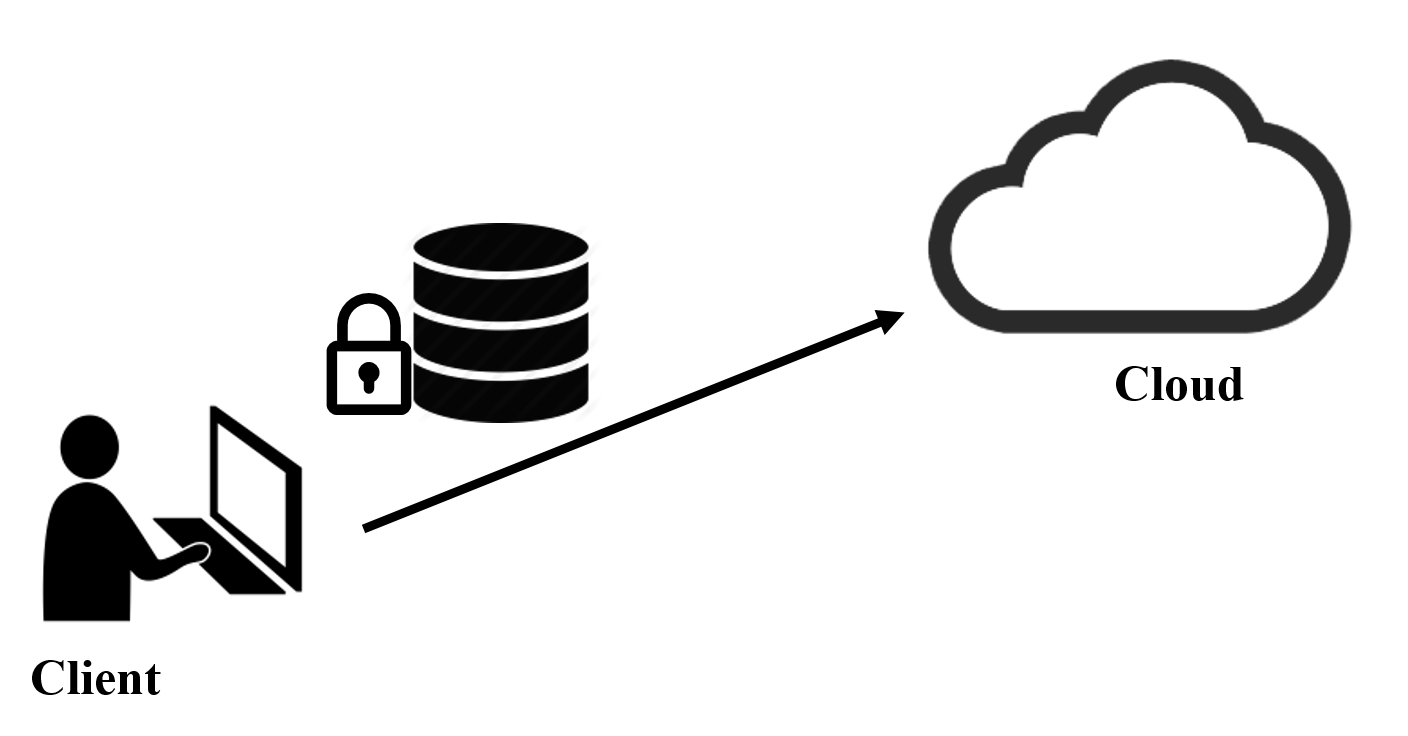
\includegraphics[width=2in]{./fig1.png}
  \caption{Outsourcing encrypted data to the cloud.}
  \label{fig_model}
\end{figure}

\subsection{Basic Searchable Encryption}

\textbf{Goals.} The description goes here.


\textbf{Design challenges.} The description goes here.

\textbf{Related work.} The description goes here.

\subsection{Dynamic Searchable Encryption}

\textbf{Goals.} The description goes here.


\textbf{Design challenges.} The description goes here.

\textbf{Related work.} The description goes here.




\subsection{Boolean Searchable Encryption}

\textbf{Goals.} The description goes here.


\textbf{Design challenges.} The description goes here.

\textbf{Related work.} The description goes here.

\subsection{Any Other Possible Categories}

\textbf{Goals.} The description goes here.


\textbf{Design challenges.} The description goes here.

\textbf{Related work.} The description goes here.

\section{Conclusion}

The conclusion goes here.


\bibliographystyle{IEEEtran}
\bibliography{references}


\end{document}
